\documentclass[3p,twocolumn]{elsarticle}
%%\usepackage[utf8]{inputenc}
%%\usepackage[LGR,T1]{fontenc}
%%\usepackage{graphicx,amsmath}
%%\usepackage[british]{babel}
%%\usepackage[latin9]{inputenc}%SOME KIND OF CLASH WITH THIS ONE
%%\usepackage{array}
%%\usepackage{rotfloat}
%%\usepackage{textcomp}
%%\usepackage{amssymb}
\usepackage{amsmath} % to align equations \usepackage{mathrsfs} % curly font in math, called using mathscr
%%\usepackage{graphicx}
%%\usepackage{subcaption} % to have two images under one caption
%%\usepackage{subscript}
%%\usepackage{gensymb} %for degree symbol
\setlength{\marginparwidth}{2cm} % to set the width of the marginpar
\usepackage{todonotes}
%%\usepackage{xargs}                      % Use more than one optional parameter in a new commands
%%\renewcommand{\baselinestretch}{1.5}
\bibliographystyle{elsarticle-num}
\begin{document}
\begin{frontmatter}
\title{Advanced Characterisation of Pore Structure in Next-Generation Reactor Graphites}
\author[plym]{Bradley Moresby-White}
\author[plym]{Katie L. Jones\corref{cor1}}
\ead{katie.jones@plymouth.ac.uk}
\author[plym]{G. Peter Matthews}
\author[plym]{Giuliano M. Laudone}
\cortext[cor1]{Corresponding author.}
\address[plym]{Faculty of Science and Engineering, University of Plymouth, Plymouth, UK}
\begin{abstract}
Nuclear grade graphite
\end{abstract}
\begin{keyword}keyword\sep keyword\sep keyword\end{keyword}
\end{frontmatter}

\section{Introduction}
This is a citation.\cite{JONES2020256HgHe}

\section{Methodology}

\subsection{Materials}

Virgin graphite samples of two grades, IG‑110 and IG‑430, were supplied by Toyo
Tanso Ltd\texttrademark, Osaka, Japan. The properties of both grades are
tabulated (Table ~\ref{tab:materialstable}).IG‑110 is currently employed in the
three existing HTGRs worldwide, while IG‑430 is designed to deliver increased
density, strength, and thermal conductivity for future
applications.\citep{toyotanso_atomic_nuclear} (Table ~\ref{tab:materialstable}).
Both grades comply with \textit{ASTMD7219-19}, including the requirement for a
minimum bulk density exceeding 1.7 g/cm$^3$ \citep{ASTMD7219-19}
(Table~\ref{tab:materialstable}).

\begin{table*}
  \centering
  \caption{Manufacturer dataset for IG-110 and IG-430 \citep{Jones2018}}
  \label{tab:materialstable}
  \resizebox{\textwidth}{!}{%
    \begin{tabular}{l l c c c c c}
      \hline
      Grade   & Coke source & Bulk density/g cm$^3$ & Filler particle size/$\mu$m) & Tensile strength/MPa & Young's modulus/GPa & Thermal conductivity/W m$^{-1}$K$^{-1}$\\
      \hline
      IG‑110  & Petrol            & 1.77                  & 10                           & 25                     & 9.8                   & 120 \\
      IG‑430  & Pitch             & 1.82                  & 10                           & 37                     & 10.8                  & 140 \\
      \hline
    \end{tabular}%
  }
\end{table*}

\subsection{Sample preparation}
Cuboids were sub-sampled from the virgin graphite blocks, with dimensions of
approximately 10mm x 10mm x 100mm. The sub-samples were further subsampled into
cuobids of side lengths ~7mm, providing 3 cuboids per grade. Samples were
polished via SiC polishing pads up to a grit size of P5000, to minimise
topographical variations induced by sample preparation that may cause artefacts
during SEM imaging or low pressure gas adsorption \citep{Fang2022,Jones2018}.Samples were
sonicated in 2-propanol for 24h to remove any contaminants, particularly the
lubricant used in the machining process. Samples were then dried under
vacuum for 12 h at $305 \pm 5\,^\circ\mathrm{C}$ using the BELPREP-vac
(MicrotracBEL, Japan) in order to remove any residual moisture introduced during
the sonication process.

\subsection{Micrograph generation}
The JEOL\texttrademark  IT510 Scanning Electron Microscope was used in the
generation of the contiguous set of individual micrographs from which the full
composite is assembled. The \textit{Image Montage} capability, within the
JEOLInScope\texttrademark  package, performed this function. The system captures
a number of micrographs, with the motorised stage moving the electron beam over
the specified area with a set overlap, with the software adjusting stigmation,
contrast, and brightness. Shifts in contrast and brightness were on the order of
< 1\% \todo{Make sure to double check that figure for ACB} and thus negligible
in affecting intensity threshold for the full composite. The full set of
parameters selected are tabulated (Table ~\ref{tab:microscopy_parameters}).

\begin{table}
  \centering
  \caption{Parameters for composite assembly captured with the JEOL IT510 SEM using Image Montage Mode}
  \label{tab:microscopy_parameters}
    \begin{tabular}{l l}
      \hline
      Parameters & Values \\
      \hline
      Magnification ($\times$)                    & 1000 \\
      Resolution ($\mu$m/px)               & 0.1 \\
      Surface area per micrograph ($\mu$m$^2$) & 12\,288 \\
      Overlap (\%)                          & 10 \\
      Micrographs per sample (n)            & 196 \\
      \hline
    \end{tabular}%
\end{table}

\subsection{Composite assembly}

The composite assembly (i.e., "stitching") stage, where the overlapping
micrographs are assembled into a single image per sample, has a significant
impact on the porosity values as incorrect fusion will misrepresent pore
structures. A stitching method based on the phase correlation approach
originally developed by Kuglin and Hines, amongst the most popular approaches to
image registration, was selected and operated as a plug-in within ImageJ
\citep{Kuglin1975, Preibisch2009}. This method represents a development of the
original phase correlation method\citep{Preibisch2009}.
	
	 A key advantage of this method is the avoidance of error propogation by
	consecutive registration steps, which is key at this scale
	\citep{Preibisch2009}. A further advantage is the sub-pixel accuracy of the
	fusion, as incorrect alignments would generate false pore diameters. The
	resulting composite micrographs showed excellent alignment with no visible
	delineation between individual micrographs, a relatively high FOV, high
	resolution, and clear distinction between porosity and bulk when examined
	closely (Figure \ref{fig:IG430C split scaled}).

	\begin{figure}
		\centering
		\includegraphics[width=0.45\textwidth]{./Media/C1-IG430c fusion cropped split scaled.jpg}
		\caption{Fully assembled SEM composite: IG-430 Sample C, 1000×  magnification,
     5 kV accelerating voltage. Bar = 250 µm.}
		\label{fig:IG430C split scaled}
	\end{figure} 

	\subsection{Computation of Channel Porosity}
\subsubsection{Intensity/Greyscale Thresholding}
	
	Intensity thresholding, where intensity refers to the value of a given pixel
	in an 8-bit micrograph, is the core of global intensity thresholding.
	Intensity thresholding determines an intensity value at which porosity and
	bulk (i.e., foregound and brackground) are distinguished. Intensity-based
	thresholding requiures the conversion of the intensity values of the pixels in
	the micrograph into a histogram of intensity, enabling the selection of an image-wide
	threshold at which different classes can be separated.

For each 8-bit micrograph \(E\) (pixel values \(0 \le E(x,y) \le 255\)), we
first compute its intensity histogram \(H(i)\) for \(i=0,1,\dots,255\).
Specifically,
\[
H(i) = \sum_{x=1}^{M}\sum_{y=1}^{N} \mathbf{1}\{E(x,y)=i\},
\]
where \(M\) and \(N\) are the image width and height (in pixels), and
\[
\mathbf{1}\{E(x,y)=i\} =
\begin{cases}
1, & \text{if the pixel at }(x,y)\text{ has intensity }i,\\
0, & \text{otherwise.}
\end{cases}
\]

For each pixel, the equation checks the intensity and increments
the count in the correspoinding bin, yielding a 256‐bin histogram whose entries
\(H(i)\) count the number of pixels at each intensity level. 

	Global automatic intensity thresholding algorithms optimising by different
	criteria to determine thresholds. For manual selection of a given threshold,
	or validation of an automatically selected threshold, there exists no certain
	criteria to allow a fully objective evaluation \citep{Huang2019}. In this
	work, thresholding aims to select an intensity value that reliably binarizes
	porosity and bulk in a way that minimizes both Type I and II errors as
	evaluated by the operator (i.e., false positives, classifying a pore where one
	is not present, and false negatives, not classifying a pore where one is
	present).

  A test of all 17 of the available automatic thresholding methods available in
   Fiji/ImageJ demonstrated that no automatic global intensity thresholding
   algorithm effectively distinguished between porosity and bulk with the
   sensitivity required to allow the classification of pores for the given
   histogram (Figure ~\ref{fig:Try All Thresholding Methods}).

   The key cause is likely the lack of a bimodal distribution in the histogram
  \todo{need to make a figure for the histogram in ImageJ}, meaning that there
  are statistically no classes to be separated, necessitating the use of a
  human-in-the-loop (HITL) approach.

	\begin{figure}[!htbp]
		\centering
		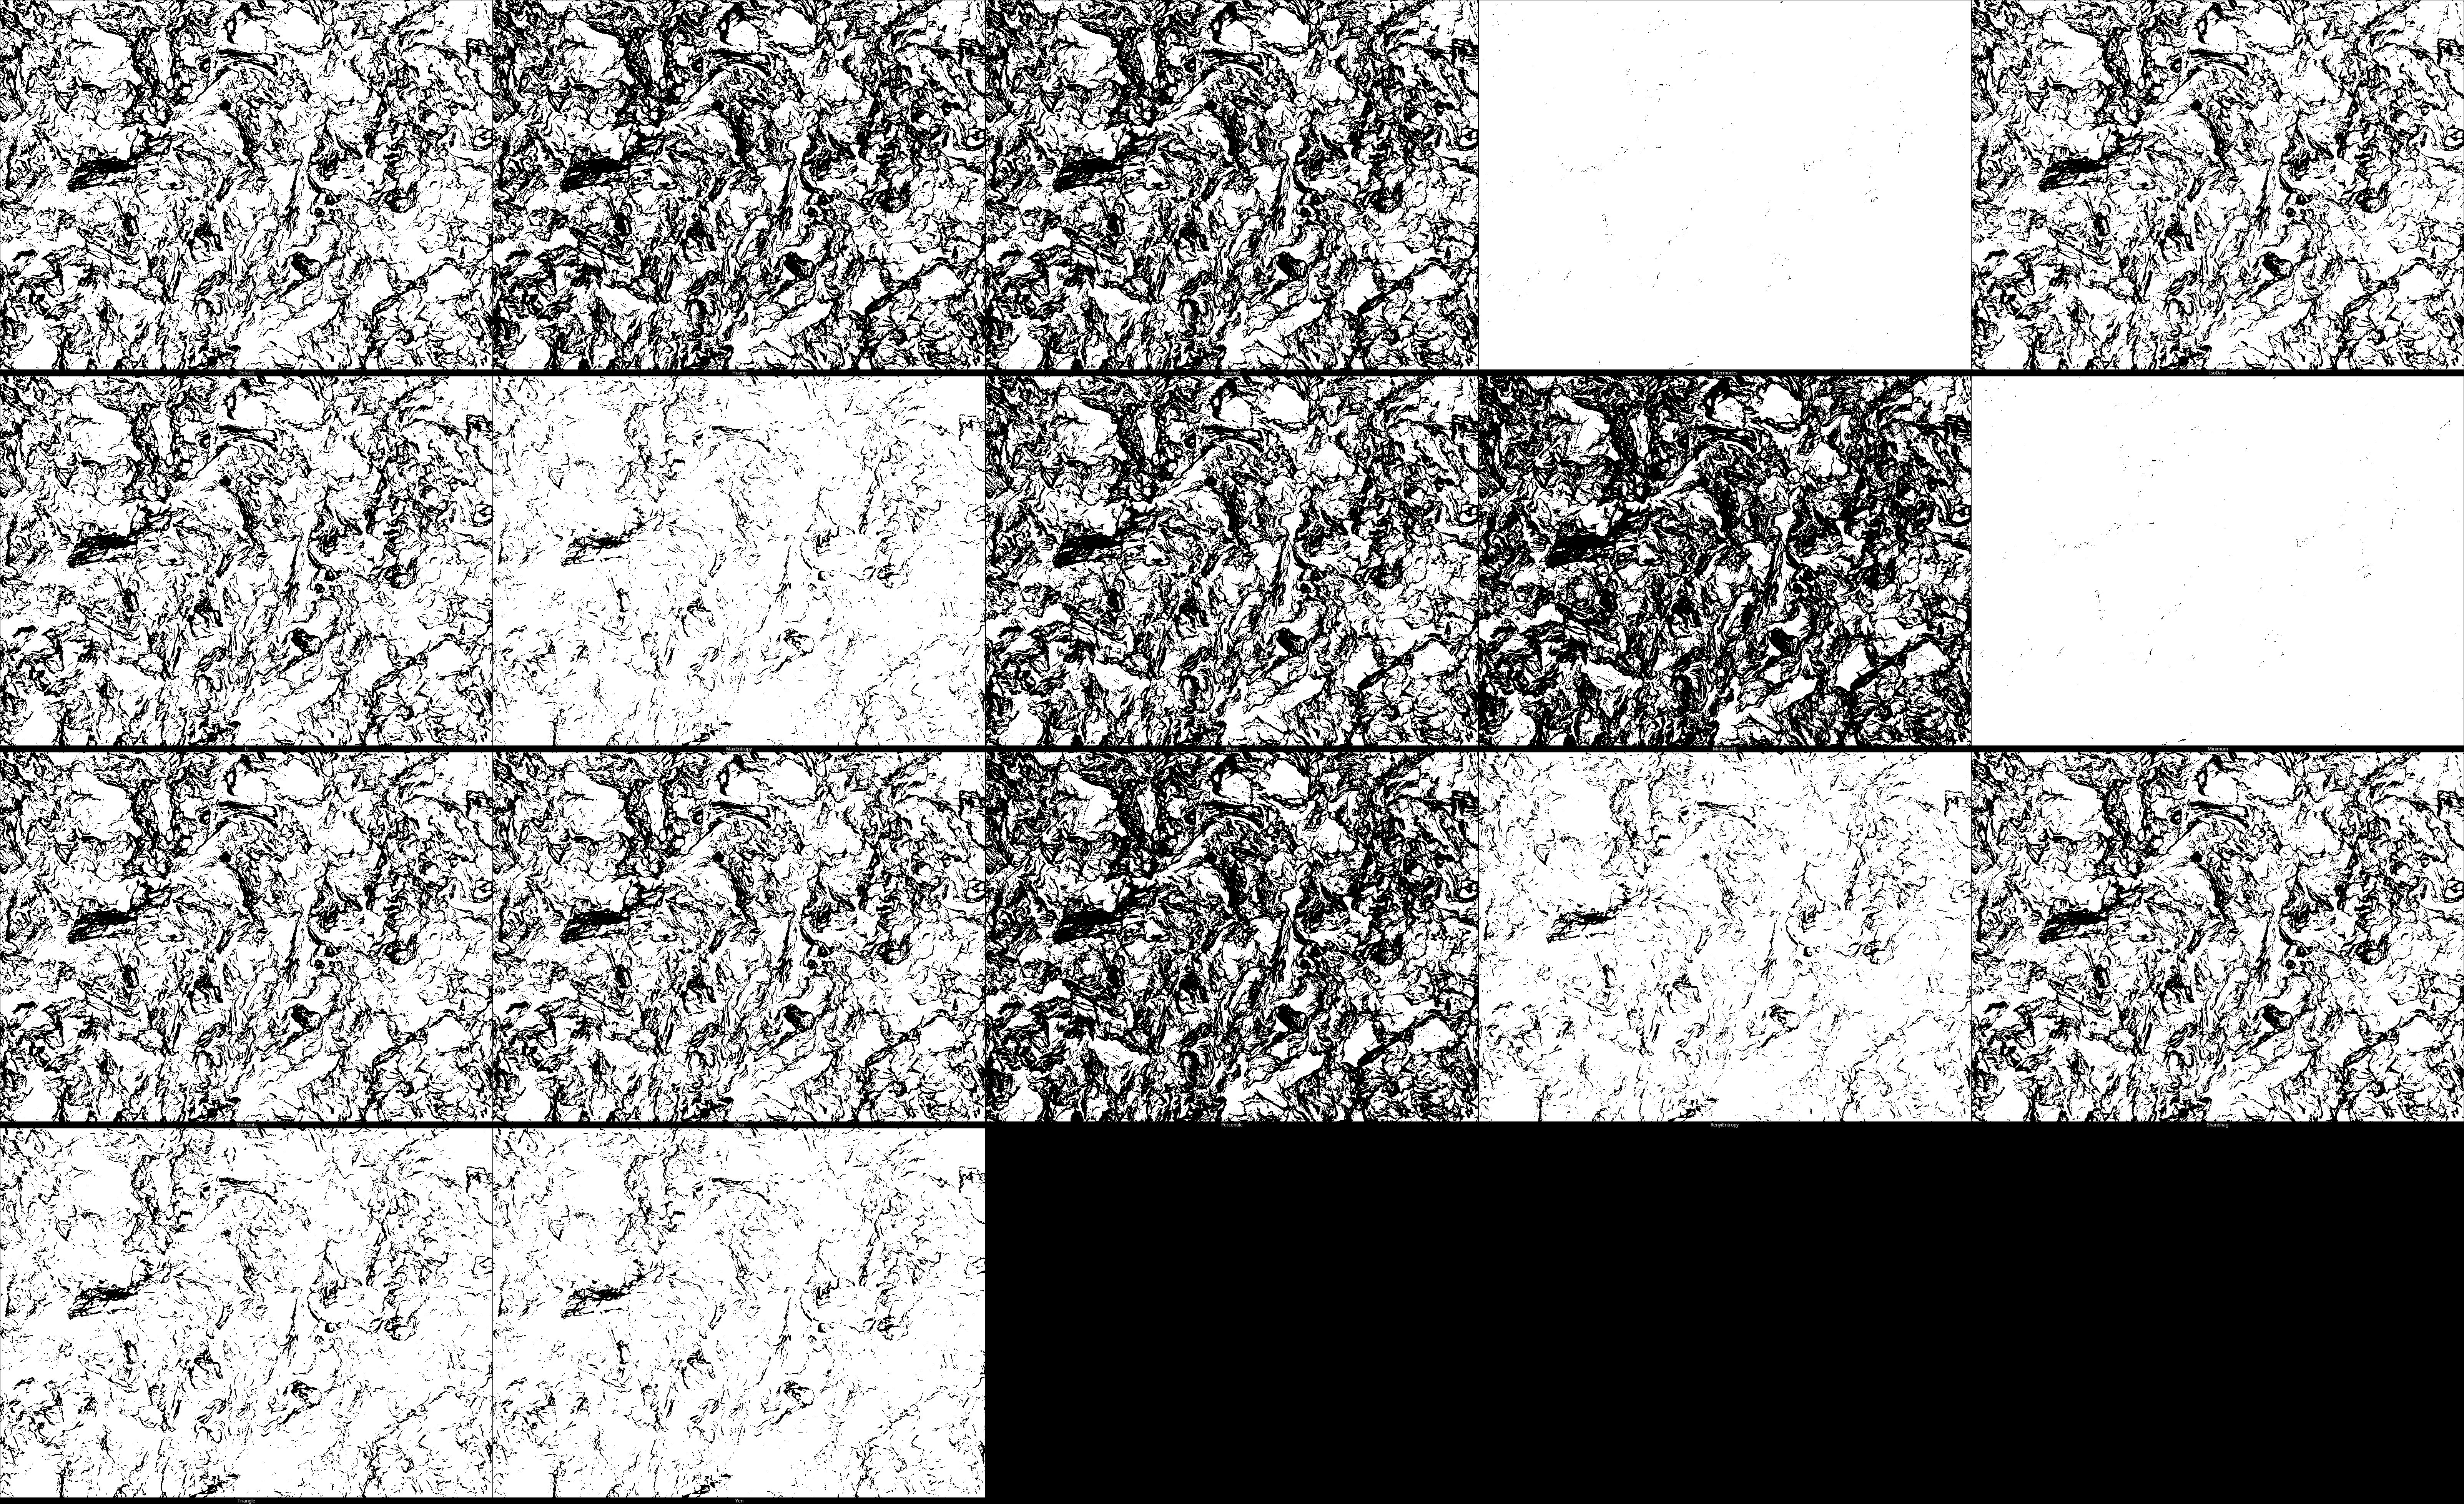
\includegraphics[width=0.45\textwidth]{./Media/MontageIG430C Methods.jpg}
		\caption{Thresholded Micrograph of IG-430 Sample C at $1000\times$ Magnification. Methods are labelled sequentially from right to left, row by row. (a) Default
			(b) Huang
			(c) Huang2
			(d) Intermodes
			(e) IsoData
			(f) Li
			(g) MaxEntropy
			(h) Mean
			(i) MinError(I)
			(j) Minimum
			(k) Moments
			(l) Otsu
			(m) Percentile
			(n) RenyiEntropy
			(o) Shanbhag
			(p) Triangle
			(q) Yen}
		\label{fig:Try All Thresholding Methods}
	\end{figure}  

	A HITL (human-in-the-loop) approach was therefore undertaken, as illustrated
	in the  process diagram through the example of IG-110 Sample B (Figure
	~\ref{fig:Final Workflow}). Here, the operator subsamples the overall fused
	compsite, then examines this subsample to determine the threshold at which
	the porosity and bulk are best separated. The operator then applies this
	threshold to the full composite, and the results are classified as either
	porosity or bulk to derive channel porosity.
	
\begin{figure}[!htbp]
    \centering
    \includegraphics[width=0.45\textwidth]{./Media/Newprocessmodel.png}
    \caption{Full thresholding workflow detailing the process of micrograph generation,
     composite assembly, subsampling, intensity thresholding, and pore diameter thresholding.}
    \label{fig:Final Workflow}
\end{figure}

	\subsubsection{Pore Diameter Thresholding}
    
   Pore diameter thresholds are imposed in this work, as in previous works, to
   constrain the automated recognition of pores to that interval within which
   classification is deemed reliable \citep{Taylor2016, Huang2019, Kane2011a}.
   The constraint on objectivity is the infeasibility of defining absolutely
   whether a given classification of a pore is correct. Even where this is done,
   at this scale it would require the comparison of classified porosity to the
   original micrograph, for thousands of pores per micrograph. 

    (Step 6, Figure ~\ref{fig:Final Workflow})  is the imposition of a pore size
      threshold via a HITL method once more, with the operator's comparison of
      the results of a range of pore diameter thresholds to the raw subsample to
      determine a specific area to be applied across the samples. The variations
      per threshold are shown in Table ~\ref{tab:thresholdsandvariations} and
      Figure \ref{fig:improvedporediademo}.
      
      Significant variation is exhibited in the number of pores characterised as
      a function of pore size threshold (Table
      \ref{tab:thresholdsandvariations}). The corresponding variation in total
      porosity is lower, 3 pores of an area greater than 8 µm\(^2\)
      in the subsample represent 46.71\% of total porosity as classified, where
      no area threshold is applied. In this work, an area threshold of 1
      µm\(^2\) (dia = 1.12 µm) has been selected as the optimal compromise between the Type I
      and Type II errors.

\begin{table}
  \centering
  \caption{Effect of different pore area thresholds on IG-110 Sample B, showing the resulting pore count, average size, total area, and estimated channel porosity.}
  \label{tab:thresholdsandvariations}
  \resizebox{\columnwidth}{!}{%
    \begin{tabular}{l c c c c c c}
      \hline
      {Area Threshold} ($\mu$m$^2$) & 0 & 0.5 & 1 & 2 & 4 & 8 \\
      Pore Count (n) & 109 & 39 & 30 & 18 & 10 & 3 \\
      Average Size ($\mu$m$^2$) & 1.709 & 4.437 & 5.554 & 8.263 & 12.611 & 29.003 \\
      Channel Porosity (\%) & 3.55 & 3.30 & 3.18 & 2.84 & 2.41 & 1.66 \\
      \hline
    \end{tabular}
  }
\end{table}

\begin{figure}[!htbp]
    \centering
    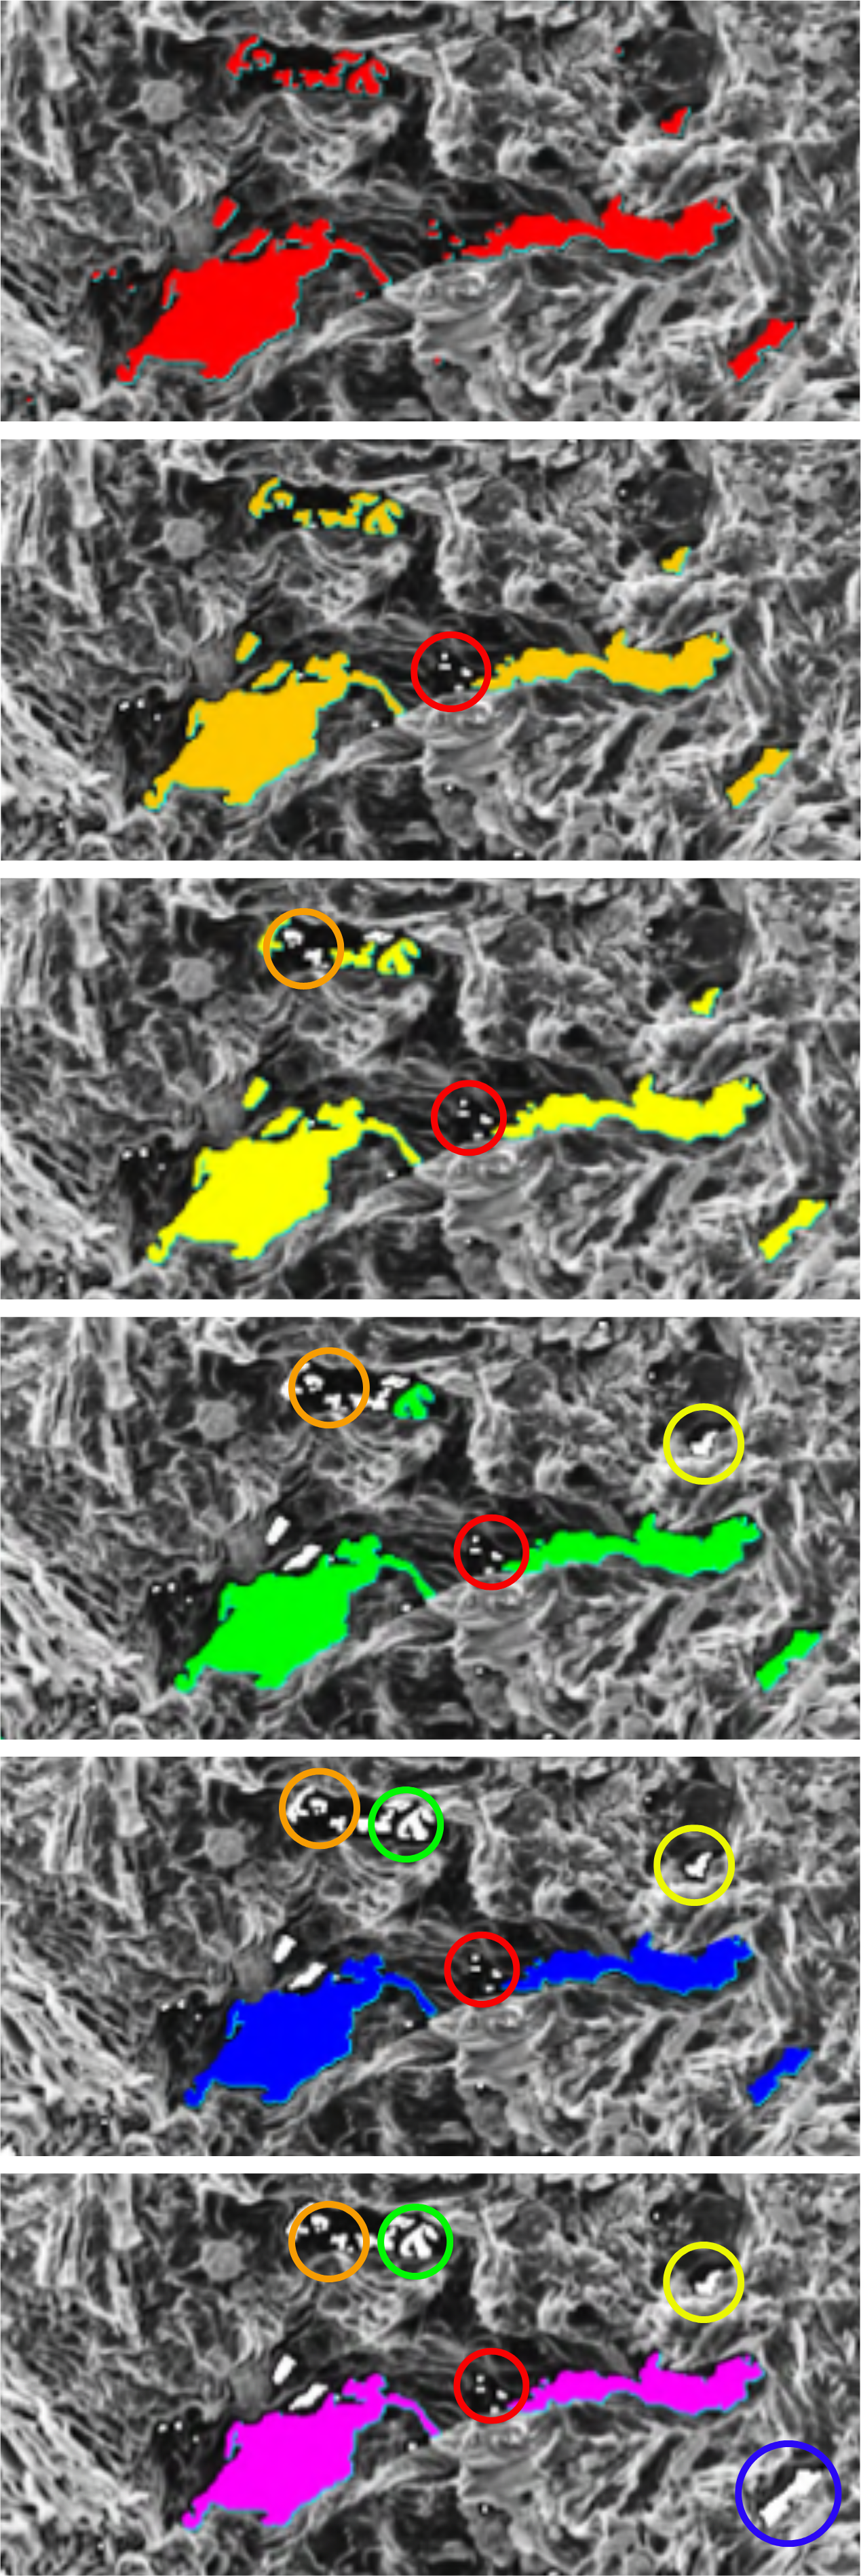
\includegraphics[width=0.35\textwidth]{./Media/ImprovedPoreDiaDemo.png}
    \caption{Effect of minimum area threshold on pore identification in subsample of IG-110 Sample B. Highlighted circles denote features which surpassed the previous threshold(s) only, indicated by colour. Thresholds applied (a–f, left-to-right, top-to-bottom): None, 0.5 µm\(^2\), 1 µm\(^2\), 2 µm\(^2\), 4 µm\(^2\), and 8 µm\(^2\).}
    \label{fig:improvedporediademo}
\end{figure}

\subsection{Helium (He) Pycnometry}
	
Skeletal density was obtained using a Pycnomatic ATC pycnometer (Thermo Fisher
Scientific, Italy) at a temperature of 20.00 ± 0.01\textdegree{}C. Measurements
were taken in ten replicates per sample, calculating the arithmetic mean.

Solid phase volume $V_{\mathrm{SOLID}}$ was calculated assuming a theoretical
density of \todo{insert theoretical density here} g cm$^{-3}$ for an ideal graphite crystal. Closed Pore Volume
(CPV) and Open Pore Volume (OPV) for each of the samples was calculated via
equations \ref{eq:CPV} and \ref{eq:OPV}.

\begin{equation}
\mathrm{CPV} = \frac{m - V_{\mathrm{SOLID}} \times \rho{_\mathrm{s}}}{\rho{_\mathrm{s}}} 	\label{eq:CPV} 
\end{equation}

\begin{equation}
	\mathrm{OPV} = V_{\mathrm{BULK}} - \mathrm{CPV} - V_{\mathrm{SOLID}}\label{eq:OPV} 
\end{equation}

Specific Pore Volume (SPV), the void volume accessible to helium per gram of
sample was calculated via Equation \ref{eq:SPV}. 

\begin{equation}
\mathrm{SPV} = \frac{1}{\rho}-\frac{1}{\rho_\mathrm{s}}\label{eq:SPV} 
\end{equation}

\subsection{Mercury (Hg) Intrusion Porosimetry}
Mercury intrusion porosimetry operates on the fundamental principle that the
pressure at which a non-wetting fluid intrudes a given pore is inversely
proportional to the diameter of that pore (i.e., the larger the pore, the easier
it is for the non-wetting fluid to enter it). The exact physical relationship
between diameter and applied pressure is governed by the following equation (Eq.
~\ref{eq:washburn})
	
	\begin{equation} \label{eq:washburn}
		d = \frac{-4\gamma \cos \theta}{P}
	\end{equation}

		The pore diameter \(d\) is calculated using the equation:
	\begin{itemize}
		\item $d$ (m): Pore diameter
		\item $\gamma$ (N/m): Surface tension of the fluid
		\item $\theta$ (degrees): Contact angle of the fluid with the surface
		\item $Papp$ (P): Pressure
	\end{itemize}

Values of 140$^{\circ}$ and 130$^{\circ}$ were used for advancing and receding
contact angles respectively, while a value of 0.480 N m$^{-1}$ was assumed for the
surface tension of mercury \citep{VANBRAKEL19811}. 

Hg intrusion porosimetry cannot capture the full range of pore sizes as pores >
89µm diameter cannot be distinguished as mercury intrudes these
pores without the application of a measurable amount of pressure, and thus the
relation fails to yield a result (Eq. \ref{eq:washburn}). For pores
>2 µm diameter, structural damage due to the triaxial compression of the
crystalline structure by intruded mercury precludes an accurate determination of
porosity at this scale by Hg intrusion porosimetry \citep{Jones2018}. Hence, the
use of GCMC to "stitch" together the pore diameter ranges covered by both Hg and
He adsorption. The pore size distribution (PSD) is generated by combining the
methods into a single set of values, which PoreXpert inversely models to
capture. 

\subsection{Nitrogen (N$_2$) Adsorption}
Low-pressure gas adsorption isotherms were obtained using a BELSORP-max
volumetric gas adsorption instrument (MicrotracBEL, Japan). 

\clearpage

\bibliography{bibliography}
\end{document}